\documentclass[12pt,a4paper]{article}

\usepackage[left=3cm,right=2cm,top=2.5cm,bottom=1.5cm,includeheadfoot]{geometry}
\usepackage[english, ngerman]{babel}
\usepackage{amsmath}
\usepackage{graphicx}
\usepackage{xcolor}
\usepackage{makeidx}

% Blindtext
\usepackage{blindtext}
\usepackage{lipsum}

% Umlaute
\usepackage[utf8]{inputenc}

% Verbesserte Schrift
\usepackage{microtype}

% Verlinkungen
\usepackage{hyperref}

% Bessere Tabellen
\usepackage{array}
%\usepackage[table]{xcolor}

% Abkürzungsverzeichnis
\usepackage[nolist, nohyperlinks]{acronym}

% Figure a b
\usepackage{subcaption}

\usepackage[style=authoryear]{biblatex}
\usepackage[T1]{fontenc}
\usepackage{lmodern}
\addbibresource{main.bib}
% !TEX root = main.tex
\hypersetup{
	pdftitle={Master-Arbeit},
	pdfsubject={Reactive Programming mit Quarkus},
	pdfauthor={Erik Simonsen},
	pdfkeywords={Reactive, Reactive Programming, Quarkus, Java},
	pdfstartpage={1},
	plainpages=false,
	hypertexnames=false
}

\usepackage{tikz-qtree}
\usetikzlibrary{positioning}

\definecolor{nodeRed}{HTML}{F44336}
\definecolor{nodeBlue}{HTML}{2196F3}
\definecolor{nodeYellow}{HTML}{FFEB3B}
\definecolor{nodeGreen}{HTML}{4CAF50}
\definecolor{nodeOrange}{HTML}{FF9800}
\definecolor{nodeGray}{HTML}{607D8B}

% Tikz Tree settings
\tikzset{every tree node/.style={draw, rectangle, minimum width=1.5em, minimum height=1.5em,line width=1pt}, level distance=1.3cm,sibling distance=0.5cm}
\tikzset{red/.style={draw, fill=nodeRed}}
\tikzset{blue/.style={draw, fill=nodeBlue}}
\tikzset{yellow/.style={draw, fill=nodeYellow}}
\tikzset{green/.style={draw, fill=nodeGreen}}
\tikzset{orange/.style={draw, fill=nodeOrange}}
\tikzset{gray/.style={draw, fill=nodeGray}}
\tikzset{white/.style={draw, fill=white}}
\tikzset{black/.style={draw, fill=black}}
% !TEX root = main.tex
\usepackage{ntheorem}
\usepackage{mdframed}

\theoremstyle{break}
\theoremheaderfont{\bfseries}
\newmdtheoremenv[
nobreak=true,
linecolor=red,
linewidth=2,
leftmargin=0,
rightmargin=0,
backgroundcolor=yellow,
innertopmargin=10pt,
ntheorem]{todo}{TODO}[section]

\begin{document}

    \pagestyle{empty}
    \pagenumbering{roman}
    \begin{minipage}{2.1cm}
	
\includegraphics[width=2cm]{resources/fh_logo_klein.jpg}
\end{minipage}
\begin{minipage}{10.0cm}
	Ostfalia - Hochschule für angewandte Wissenschaften\\
	Fakultät Informatik\\
	Institut für Software Engineering
\end{minipage}

\vspace{35mm}

\begin{center}
	{\LARGE Master-Arbeit}
	\\[10mm]
\end{center}

\begin{center}
	\LARGE \textbf{Reactive Programming mit Quarkus\\[28mm]}
\end{center}

\begin{table}[h]
	\centering
	\hspace{50mm}\begin{tabular}{lcll}
		eingereicht von &  & Erik Simonsen           & 70455429 \\

		Erstprüfer:     &  & Prof. Dr. B. Müller     &          \\
		Zweitprüfer:    &  & Prof. Dr. H. Grönninger &          \\
	\end{tabular}
\end{table}

\vspace{30mm}

\begin{table}[h]
	\begin{tabular}{lll}
		Wolfenbüttel, den \today \\
	\end{tabular}
\end{table}
\clearpage

    \begin{abstract}
    \normalsize
    \noindent
    Das Ziel der vorliegenden Masterarbeit ist es, das Konzept von reaktiver Programmierung und reaktiven Systemen,
    speziell im Java Ökosystem, zu erläutern. Zudem wird untersucht, ob eine reaktive Anwendung nach dem \verb|Reactor Pattern| das, durch
    Threadwechsel bedingte, Skalierungsproblem einer nicht-reaktiven, auf dem \verb|Thread per request|-Pattern basierenden,
    Anwendung bei hohen Lasten lösen kann.\newline

    Dafür wurden in einem Versuchsaufbau eine Reihe von Lasttests mit stetig steigenden Lasten, jeweils mit und ohne Datenbankanbindung,
    an zwei konzeptionellen Anwendungen,
    reaktiv und nicht-reaktiv, durchgeführt. Dabei wurden leistungsrelevante Metriken wie Durchsatz, Speicherbedarf und CPU-Auslastung gemessen.
    Anschließend wurden die Ergebnisse beider Anwendungen ausgewertet und miteinander verglichen.
    Beide Anwendungen wurden dabei mit dem Full-Stack, Kubernetes-nativen Java-Anwendungsframework \verb|Quarkus| implementiert.\newline

    Die Auswertung der Messergebnisse zeigt, dass die reaktive Anwendung sowohl beim Arbeiten mit statischen, als auch dynamischen Daten
    mit Datenbankanbindung in jeder gemessenen Metrik, besonders im Durchsatz, der nicht-reaktiven Anwendung überlegen ist.
    Bezüglich der Verständlichkeit, Wartbarkeit und Integrationsfähigkeit ist sie nach Auffassung des Autors gegenüber
    einer nicht-reaktiven, traditionellen Anwendung jedoch im Nachteil.
    Die Testergebnisse sind außerdem durch eine Vielzahl
    an Faktoren, wie Hardwareleistung oder Datenbankgröße, beeinflussbar, weswegen der Autor empfiehlt die Testumgebung
    an die eigenen Anforderungen anzupassen.
    Darüber hinaus werden Alternativen zum reaktiven Modell im Java-Umfeld dargestellt und bewertet.\newline

    Weiterführende Arbeiten in diesem Bereich könnten die genannten Metriken von alternativen Ansätzen, wie der Nutzung von virtuellen Threads durch Project Loom,
    in einem ähnlichen Versuchsaufbau untersuchen und mit einer reaktiven Anwendung vergleichen.
\end{abstract}

    \clearpage
\thispagestyle{empty}

\section*{Ehrenwörtliche Erklärung}

Hiermit erkläre ich ehrenwörtlich, dass ich die vorliegende Arbeit selbstständig und ohne unerlaubte fremde Hilfe angefertigt habe, andere als die angegebenen Quellen nicht benutzt und die  benutzten Quellen wörtlich oder die inhaltlich entnommenen Stellen als solche kenntlich gemacht habe.
\vspace{4em}\\
Wolfenbüttel, den \today

    % !TEX root = main.tex
\clearpage
\tableofcontents
    % !TEX root = main.tex
\clearpage
\listoffigures
\clearpage
%% !TEX root = main.tex
\section*{Stichwortverzeichnis}
\label{sec:Stichwortverzeichnis}
\begin{acronym}
    \acro{ecu}[ECU]{European currency unit} Test
    %ToDo: On-Demand Streaming, Live-Streaming, Webkonferenz
\end{acronym}
%% !TEX root = main.tex
\section*{Abkürzungsverzeichnis}
\label{sec:Abkürzungsverzeichnis}
\begin{acronym}
    \acro{ecu}[ECU]{European currency unit} Test
    %ToDo: On-Demand Streaming, Live-Streaming, Webkonferenz
\end{acronym}

    \setcounter{page}{1}
    \pagenumbering{arabic}
    \pagestyle{headings}

    \section{Einleitung}
\label{sec:einleitung}
In der folgenden Arbeit sind die ersten Vorkommen von möglicherweise nicht geläufigen Begriffen und Abkürzungen, die
im Fließtext nicht erklärt werden, mit einem \verb|(*)| gekennzeichnet.
Diese Begriffe werden im Glossar und/oder Akronymverzeichnis kurz erklärt.

\subsection{Problemstellung}
\label{subsec:problemstellung}
In den letzten Jahren sind die Anforderungen an Webanwendungen durch zunehmende Digitalisierung und entsprechend steigenden Nutzerzahlen,
sowie stark auf Client-Server Kommunikation basierenden Architekturen, wie Microservices und \Glspl{spag}(*), erheblich gestiegen.

Während geschäftskritische Anwendungen lange Zeit mit ein paar Tausend Anfragen pro Sekunde als hoch frequentiert
galten, müssen solche Webanwendungen heutzutage in der Lage sein eine vielfach höhere Last bewältigen zu können.
Darüber hinaus müssen sie \verb|skalierbar| sein, also ohne Leistungseinbußen auf variable Lasten reagieren können.

Das Standardmodell für Java-basierte Webanwendungen ist das \verb|Thread per request|-Modell.
Dabei wird jede HTTP-Anfrage an einen Kernel-Thread gebunden, welcher anschließend die Anfrage sequentiell abarbeitet.
Damit eine möglichst hohe Anzahl an Anfragen parallel abgearbeitet werden kann, wird jedem Thread nur ein Teil der verfügbaren
CPU-Rechenzeit eines CPU-Kerns zugewiesen. Sobald die Rechenzeit eines Threads abgelaufen ist, oder er durch einen blockierenden
Funktionsaufruf in einen inaktiven Zustand versetzt wird, wird der nächste Thread bearbeitet: es erfolgt ein \verb|Threadwechsel|.

Obwohl Threadwechsel, im Gegensatz zu Prozesswechseln, sehr kostengünstig sind, sind sie in diesem Modell ab einer kritischen Anzahl von HTTP-Anfragen
pro Sekunde der begrenzende Skalierungsfaktor. Die Threadwechsel zwischen den Kernel-Threads des Betriebssystems erfolgen dann nicht mehr
schnell genug um jede Anfrage bzw. jeden Thread innerhalb einer akzeptablen Zeit zu bearbeiten.
Diese Begrenzung äußert sich letztendlich darin, dass der \Gls{durchsatz}(*) der Anwendung nicht ausreichend skaliert.

\subsection{Ziel der Arbeit}
\label{subsec:ziel}
Um höhere Workloads zu bewältigen und Anwendungen skalierbarer zu machen, existieren alternative
Anwendungsmodelle, wie das in dieser Arbeit thematisierte \verb|Reactor-Pattern|.
Das Modell nutzt einen Thread pro CPU-Kern und verzichtet somit auf anwendungsbedingte Threadwechsel.
Die Voraussetzung dafür ist allerdings, dass die vorhandenen Threads niemals in einen inaktiven Zustand geraten.
Deswegen dürfen Anfragen an externe Komponenten, wie Datenbanken oder Webservices, den Thread nicht blockieren,
und der vom Ergebnis abhängige Code muss reaktiv, also erst beim tatsächlichen Eintreffen der Antwort,
ausgeführt werden: man spricht von \verb|reaktiver Programmierung|.
Reaktive Programmierung erfordert, dass die Programmlogik jeder
Anwendungsschicht asynchron und eventbasiert strukturiert wird.
Nachdem eine Anfrage an eine externe Komponente abgesetzt wurde, beginnt der Thread bereits mit der Abarbeitung der nächsten
HTTP-Anfrage. Sobald ein Resultat verfügbar ist, wird es dem Thread mithilfe eines Events mitgeteilt.
Dieser führt daraufhin den, für dieses Event hinterlegten, Code aus. Durch diese grundlegende Funktionsweise wird auf anwendungsbedingte
Threadwechsel verzichtet.

In dieser Arbeit wird untersucht, ob \verb|Reactive Programming| bzw. reaktive Anwendungen das Problem der Skalierbarkeit
für hohe Lasten praktikabel lösen können und welche alternativen Lösungsansätze es gibt.

\subsection{Vorgehensweise}
\label{subsec:vorgehensweise}
Um das Verhalten der beiden Modelle unter Last zu prüfen und miteinander zu vergleichen, werden zwei triviale Anwendungen implementiert,
reaktiv und nicht-reaktiv, und einer Reihe von Lasttests mit unterschiedlichen \verb|workloads| unterzogen.
Dabei werden verschiedene \Glsplural{benchmark}(*), wie Durchsatz, Speicherbedarf und CPU-Auslastung gemessen.
Die Anwendungen werden sowohl auf der \acrshort{jvm}(*), als auch nativ ausgeführt und jeweils mit und ohne Datenbankenanbindung getestet.

\subsection{Aufbau}
\label{subsec:aufbau}
Zu Beginn der Arbeit werden in Kapitel \ref{sec:grundlagen} die Grundlagen der Thematik erläutert. Diese beinhalten
Kernel- und User-Threads, blockierende und nicht-blockierende Ein-/Ausgabe-Operationen sowie die beiden darauf aufbauenden Design-Patterns
\verb|Thread per request| und \verb|Reactor|.

Anschließend wird in Kapitel \ref{section:reaktive_programmierung} die Funktionsweise von \verb|Reactive Programming|, und dessen
zugrundeliegendes Konzept von reaktiven Datenströmen erläutert. Danach werden die Vor- und Nachteile des Programmierparadigmas
genannt.
Darauffolgend werden die Eigenschaften von reaktiven Systemen und deren Beziehung untereinander beschrieben.
Zum Ende des Kapitels wird auf die Unterstützung für reaktive Anwendungen und Architekturen innerhalb des Java Ökosystem
sowie Alternativen eingegangen.

In Kapitel \ref{section:vergleich_reaktiv_blockierend} wird zuerst die Testumgebung definiert sowie Testaufbau und Testablauf beschrieben.
Im Anschluss werden die Testresultate genannt und in Form von Diagrammen dargestellt.
Abschließend erfolgt die Auswertung und Erläuterung der Testresultate.
    \newpage
    \input{mainmatter/vergleich_streaming_ansätze}
    % !TEX root = main.tex

\section{System}
\label{sec:system}
%In diesem Kapitel werden die wesentlichen Komponenten der Implementierung erläutert.
%
%Die Aufnahme der Medienquellen wird durch die getUserMedia-API über das \textit{MediaStream}-Objekt ermöglicht.
%ToDo

\subsection{WebSockets}
\label{subsec:websockets}
Für das Signaling ist eine Kommunikation über mehrere Schritte hinweg notwendig.
Damit diese ohne eine Vielzahl an HTTP-Anfragen und komplexer serverseitiger Vorkonfiguration realisiert werden können, wird client- und serverseitig
die WebSocket-API\parencite{WebSocketSpec} genutzt\footnote{Serverseitig wird die WebSocket API von Java genutzt\parencite{JavaEEWebSocket}}.
Da WebRTC allerdings keinen Transport-Mechanismus für die Signaling-Informationen spezifiert, ist es auch möglich die Informationen über
XMLHttpRequests zu versenden (sog. Ajax-Requests).
WebSockets ermöglichen die bidirektionale Client-Server Kommunikation.
Dabei kann der Client dem Server Nachrichten senden und ereignisorientierte Antworten erhalten,
ohne Antworten durch HTTP-Anfragen abzufragen\parencite{WebSocketMDN}.
Die Nachrichten werden dabei im JSON-Format ausgetauscht.
Folgende Ereignisse können, sowohl client- als auch serverseitig, ausgelöst werden:
\begin{itemize}
    \item OnOpen()
    \item OnMessage()
    \item OnClose()
    \item OnError()
\end{itemize}

\subsection{SDP (Session Description Protocol)}
\label{subsec:sdp}
SDP ist ein Standardformat um eine \textit{peer-to-peer} Verbindung zu beschreiben und wird u.A. von WebRTC genutzt um Sitzungen von \textit{peers} zu beschreiben.
Es enthält Informationen zur verwendeten Codec, den IP-Adressen der \textit{peers}, und zu Zeitabschnitten von Video- und Audiodaten\parencite{MDNSdp}.
\begin{figure}[!ht]
%figure full paperwidth and trim the left and right empty space from it
    \makebox[\textwidth]{
        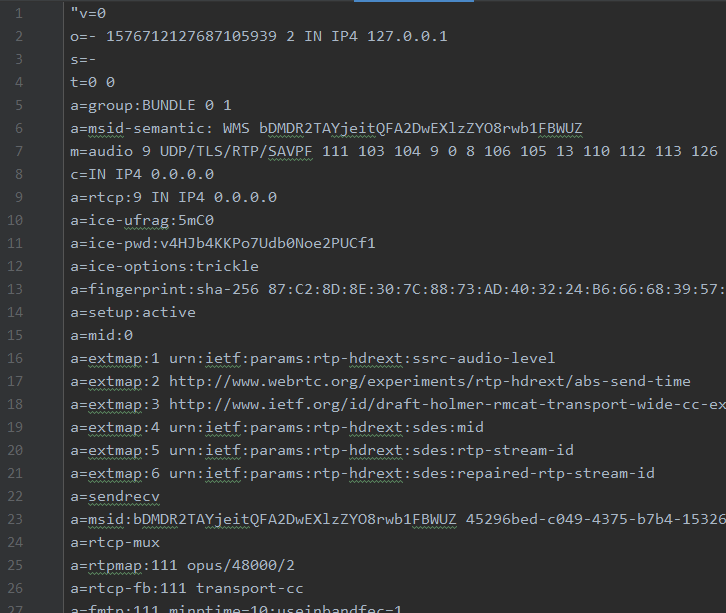
\includegraphics[trim = 16mm 0mm 16mm 0mm,width=0.7\paperwidth]{resources/sdp-localhost-example.png}
    }
    \caption{Ausschnitt einer SDP-Nachricht zwischen zwei \textit{peers} auf \textit{localhost}}
    \label{fig:sdp-localhost}
\end{figure}

\subsection{ICE (Interactive Connectivity Establishment)}
\label{subsec:ice}
ICE ist ein von WebRTC genutztes Framework um zwei Peers miteinander zu verbinden, unabhängig von der vorhandenen Netzwerk-Topologie. \parencite{RFCIce}
Das ICE-Protokoll ermöglicht das finden und etablieren einer Verbindung zwischen zwei \textit{peers}, selbst wenn beide eine Netzwerkadressübersetzung(NAT)
nutzen, um eine öffentliche IP Adresse mit anderen Geräten in ihrem Netzwerk zu teilen.
Dafür kann im Konstruktor eines RTCPeerConnection-Objektes ein STUN und/-oder TURN Server angegeben werden.

Der Algorithmus des Frameworks versucht dabei immer den Pfad mit der niedrigsten Latenz zu nutzen um die beiden \textit{peers} zu verbinden.
Dabei probiert er die folgenden Optionen in der genannten Reihenfolge:

\begin{enumerate}
    \item Direkte UDP Verbindung (in diesem Fall wird ein STUN Server genutzt um die IP-Adresse des \textit{peers} innerhalb des Netzwerkes zu finden)
    \item Direkte TCP Verbindung, über den HTTP-Port
    \item Direkte TCP Verbindung, über den HTTPS-Port
    \item Indirekte Verbindung über einen TURN Server (wenn eine direkte Verbindung fehlschlägt, bspw. wenn ein \textit{peer} hinter einer
    Firewall liegt, die die NAT-Traversierung blockiert)\parencite{MDNIce}
\end{enumerate}

\subsection{STUN und TURN Server}
\label{subsec:natturnserver}
STUN (Session Traversal Utilities for NAT) ist ein Hilfsprotokoll um Daten durch ein NAT (Network Address Translator) an das Ziel zu übermitteln.
Es gibt die IP-Adresse, den Port, und den Verbindungsstatus des Computers hinter dem NAT zurück\parencite{MDNStun} und ermöglicht somit
eine direkte Kommunikation der beiden \textit{peers}.
\newline
TURN (Traversal Using Relays around NAT) ist ein Protokoll das einem Computer - hinter einem NAT oder einer Firewall - ermöglicht Daten zu senden und empfangen.
Dabei wird der gesamte Traffic der beiden \textit{peers} während den \textit{gesamten} Kommunikationszeitraums über den TURN-Server an den jeweils anderen \textit{peer} weitergeleitet.
Der TURN-Server muss dabei in der Regel öffentlich zugänglich sein.
TURN-Server werden dann genutzt, wenn eine direkte Kommunikation der \textit{peers} durch eine sehr restriktive Firewall nicht möglich ist\footnote{
    Bei permanent hohem Traffic der \textit{peers} kann die Nutzung eines externen TURN-Servers ein Performance-Bottleneck darstellen.}\parencite{MDNTurn}.

\subsection{Signaling}
\label{subsec:signaling}

Ein Signaling-Server fungiert als Mittelsmann und ermöglicht es zwei \textit{peers} sich zu finden und eine Verbindung aufzubauen, indem
er die Signaling-Daten jeweils an den entsprechenden {peer} weiterleitet.
Dabei muss der Server den Inhalt der Signaling-Nachrichten nicht verstehen
\footnote{Der Inhalt der Signaling-Nachrichten kann daher als Black-Box gesehen werden.} können, solange
der jeweilige \textit{peer} die Nachricht erhält und an sein ICE-System (siehe Abschnitt \textit{ICE}) weitergibt.
WebRTC nutzt für die Inhalte der Signaling-Nachrichten das \textit{Session Description Protocol (SDP)} und
für die Kommunikation mit dem Signaling-Server werden \textit{WebSockets} empfohlen.

Zu Beginn des Signaling Prozesses initialisiert Peer A ein RTCPeerConnection-Objekt und erstellt ein Offer mithilfe der CreateOffer()-Methode.
Das Offer enthält seine Session-Description im SDP-Format und wird über den Signaling-Server an Peer B geschickt, welcher auch ein RTCPeerConnection erstellt.
Dieser verarbeitet das Offer und dessen Inhalt und reagiert mit einer Answer, die wiederrum die Session Description von Peer B enthält.

Nachdem Peer A die Answer verarbeitet hat, haben beide \textit{peers} das jeweilige RTCPeerConnection-Objekt mit ihrer und der Session-Description des anderen
Peers gefüllt, sowie den Audio-und Videodaten der jeweiligen Medienquelle als MediaStream-Objekt.

Beide \textit{peers} kennen nun die IP-Adresse des jeweils anderen und die zu nutzenden Codecs, wissen noch allerdings nicht wie die
Mediendaten übertragen werden sollen.
Um dies zu ermitteln, wird das ICE-Framework von WebRTC genutzt.

\begin{figure}[!ht]
%figure full paperwidth and trim the left and right empty space from it
    \makebox[\textwidth]{
        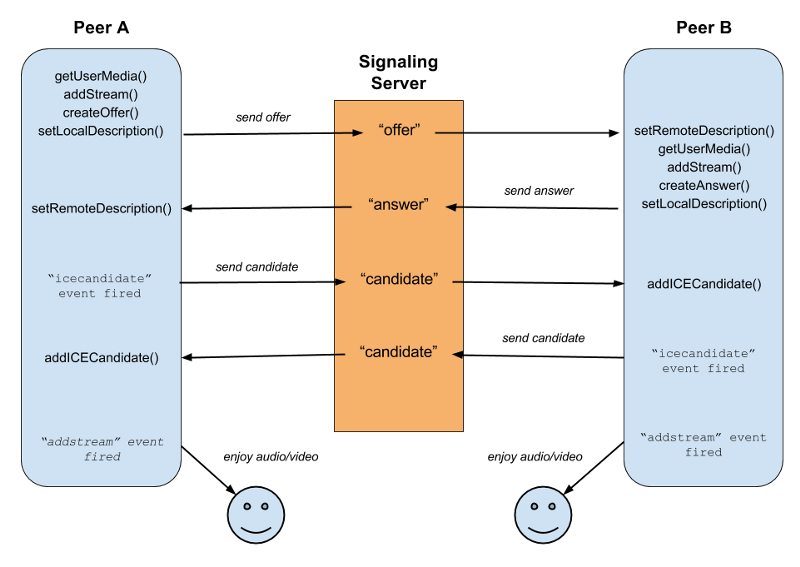
\includegraphics[trim = 16mm 0mm 16mm 0mm,width=0.8\paperwidth]{resources/WebRTC-Signaling.png}
    }
    \caption{WebRTC Signaling Ablauf, \parencite{SatanasGithub}}
    \label{fig:webrtc_signaling}
\end{figure}

Die \textit{peers} tauschen ICE-Kandidaten aus um die aktuelle Verbindung zu verhandeln.

Jeder ICE-Kandidat beschreibt eine Methode die der sendende \textit{peer} zur Kommunikation nutzen kann.

Beide \textit{peers} senden Kandidaten in der Reihenfolge, in der sie entdeckt werden, und senden solange bis sie keine Vorschläge
mehr haben - selbst wenn die Mediendaten bereits übertragen werden.
Jede ICE-Nachricht schlägt ein Kommunikationsprotokoll (TCP oder UDP), IP-Adresse, Port und andere Informationen vor, die benötigt werden
um eine Verbindung aufzubauen.
Dies beinhaltet auch NAT .

Sobald sie sich auf einen beidseitig-kompatiblen Kandidaten geeinigt haben, wird das SDP des Kandidaten von jedem Peer genutzt um eine
Verbindung aufzubauen, durch welche die Mediendaten ausgetauscht werden.

Falls Sie sich später auf einen besseren Kandidaten (normalerweise mit besserer Performance) einigen, ändert sich das Format des Datenstroms.

\parencite{MDNSignaling}


    \newpage
    % !TEX root = main.tex


\section{Implementierung}
\label{sec:implementierung}
%ToDo
%verweis auf github/gitlab link zum Projekt

\subsection{getUserMedia}
\label{subsec:getUserMedia}
Zu Beginn der Anwendung wird die Wiedergabequelle des Clients in Form eines MediaStream-Objektes abgerufen.
Die Umsetzung ist durch die \textit{getUserMedia-API()} sehr einfach und beschränkt sich auf wenige Zeilen-Code.

Hierbei wird der Benutzer aufgefordert dem Browser Zugriff auf eine Medienquelle zu gewähren, die einen MediaStream produziert der die angegebenen
Medientypen (Video und Audio) als Spuren (\textit{MediaStreamTrack}) enthält.
Anzumerken ist hierbei das die Methode \textit{getUserMedia()} asynchron ist.
Für die Nutzung der API außerhalb der lokalen Entwicklung (localhost) muss die Anwendung zudem über
HTTPS geladen werden (\textit{secure context}) \parencite{MozUserMediaSecurity}.

Nachdem dies erfolgt ist beginnt der Signaling-Prozess.

\subsection{Signaling}
\label{subsec:Signaling}
Für den Austausch der notwendigen Signaling-Nachrichten werden client- und serverseitig WebSockets verwendet.
Clientseitig wird dafür die WebSocket-API genutzt und einfach über \textit{new WebSocket()} das Objekt erstellt.
Serverseitig wird die Java-API für WebSocket (JSR 356) genutzt und mit der \textit{@ServerEndpoint} Annotation ein Endpunkt erstellt.

Da es sich bei der entwickelten Anwendung nicht nur um einen Videochat zwischen zwei \textit{peers} handelt, sondern jeder \textit{peer}
mit einer Vielzahl an anderen \textit{peers} (n:m Beziehung) kommunizieren muss, müssen client- und serverseitig die Teilnehmer mitgeführt werden.
Im Browser wird dafür ein Array an RTCPeerConnection-Objekten verwaltet und auf dem Signaling-Server eine Menge an HttpSession-Objekten.

Sobald nun ein neuer Client ein WebSocket-Verbindung zu dem Server-Endpunkt aufbaut wird beiderseits das onOpen()-Event ausgelöst.
Der Server fügt ein neues HttpSession-Objekt hinzu, und informiert alle bestehenden Clients über die neue Verbindung, sowie den neuen Client
über alle bestehenden Clients.

Anschließend legt jeder bestehende Client ein neues RTCPeerConnection-Objekt an und erstellt ein Offer über \textit{createOffer()}, also
eine Nachricht mit der eigenen Session-Description und schickt diese an den Signaling-Server.
Der neue Client muss für jeden bestehenden Client eine neue RTCPeerConnection erstellen und auf die Offers der anderen Clients warten.
Nun wird der Kommunikationsaufbau analog zu \autoref{fig:webrtc_signaling} ausgeführt.


\begin{figure}[h]
    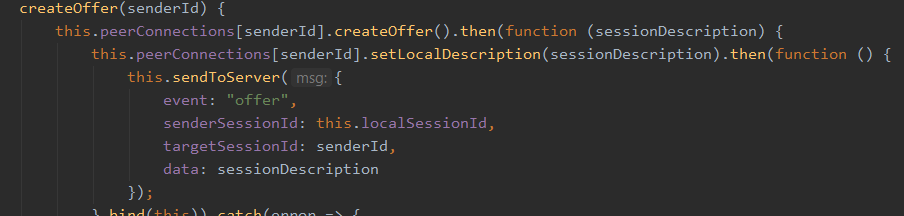
\includegraphics[width=1\textwidth]{resources/createOfferBeispiel.png}
    \caption{Codeausschnitt CreateOffer()-Methode}
    \label{fig:createOffer}
\end{figure}

Bei jeder Nachricht während des Signaling-Prozesses muss immer die Session-ID des Senders und des Empfängers angegeben werden, damit
der Server die Weiterleitung an den entsprechenden Client abwickeln kann, und der Empfänger die Nachricht dem entsprechenden
RTCPeerConnection-Objekt des Senders zuordnen kann.
Zusätzlich muss immer ein Nachrichten-Typ übermittelt werden, damit der Empfänger weiß wie er das SDP der Nachricht verarbeiten muss und wie er antworten muss.
Dafür muss im clientseitigen onMessage Event des WebSockets eine Differenzierung, je nach empfangenen Nachrichten Typ erfolgen.
\newpage

\subsection{UI}
\label{subsec:DatenaustauschUI}
Nachdem sich beide \textit{peers} auf einen ICE-Kandidaten geeinigt haben, und somit die Medien-Daten austauschen können,
wird das \textit{onTrack}-Event der \textit{peers} ausgelöst\footnote{Die addTrack()-Methode löst das onTrack-Event des RTCPeerConnection-Objektes
auf der Remote Seite aus, nicht bei dem lokalen RTCPeerConnection-Objekt}.
Die MediaStreamTrack-Objekte werden den RTCPeerConnection-Objekten bereits nach deren Initialisierung zugewiesen, sofern dann schon ein MediaStream-Objekt
vorhanden ist.

\begin{figure}[h]
%figure full paperwidth and trim the left and right empty space from it
    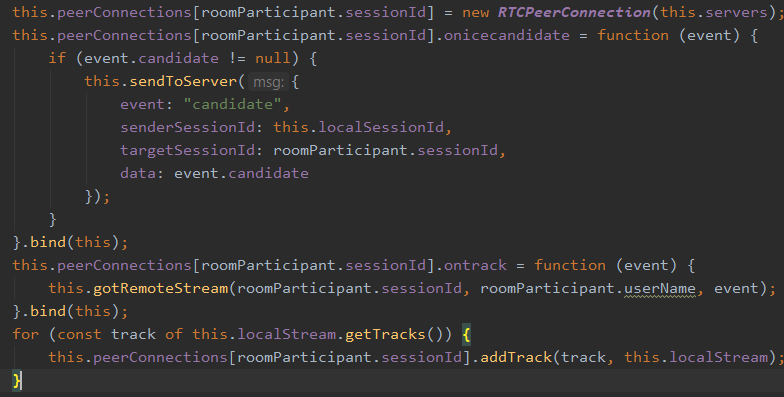
\includegraphics[width=1\textwidth]{resources/mediaStreamTracks.png}
    \caption{Codeausschnitt Datenaustausch}
    \label{fig:Datenaustausch}
\end{figure}

Im Event-Handler des \textit{onTrack }-Events kann nun auf den übertragenen MediaStream, und dessen Tracks, des anderen \textit{peers} zugegriffen werden.
Für die Oberfläche dieser Anwendung wird im Event-Handler eine Funktion aufgerufen in der für jeden neuen MediaStream ein
HTMLVideo-Element erstellt, und mit der \textit{append()}-Methode in den DOM eingefügt, wird.
Da das HTMLVideo-Element das HTMLMedia-Element-Interface implementiert kann als Wiedergabe-Quelle ein
MediaStream-Objekt gesetzt werden\parencite{WebDocsSrcObject}.

\newpage

\subsection{WebComponent}
\label{subsec:webcomponent}
Um eine möglichst hohe Wiederverwendbarkeit und leichte Anpassung für andere Projekte zu ermöglichen,
wurde die clientseitige Logik als sogenannte WebComponent gekapselt.
Dabei handelt es sich um ein benutzerdefiniertes HTML-Element, welches mit einer Javascript-Klasse verknüpft ist und
die dort definierte Funktionalität über die zu implementierende Methode \textit{connectedCallback()} ausführt sobald es vom DOM
mit dem Dokument verbunden wird.
Die Verknüpfung des <video-conference>-Elementes mit der VideoConference-Klasse wird durch die CustomElementRegistry.define()-Methode registriert.
Die VideoConference-Klasse muss zudem von der HTMLElement-Klasse erben.
Wenn die Logik nun in einem anderen Projekt für Videokonferenzen verwendet wird, kann
der Endpunkt des Signaling-Servers über die HTML-Attribute \textit{socketHostname} und \textit{socketPathname} modifiziert werden, ohne den Javascript-Code
anpassen zu müssen.
Die Existenz und der Wert dieser Attribute wird in der connectedCallback()-Methode abgefragt.
\begin{figure}[h]
    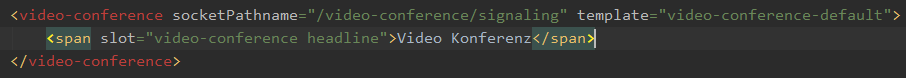
\includegraphics[width=1\textwidth]{resources/customElement.png}
    \caption{Codeausschnitt Custom <video-conference>-Element}
    \label{fig:CustomElement}
\end{figure}

Um zudem die Element-Struktur, das Styling und das Verhalten vom restlichen Code der Anwendung abzugrenzen wird
die Shadow DOM API genutzt.
Dabei handelt es sich um einen versteckten separaten DOM der an ein Element angehangen wird und nicht
von den Styles und definierten Verhalten des Standard-DOMs betroffen \parencite{WebDocsShadowDOM}.

    \newpage
    \section{Fazit}
\label{sec:fazit}

\subsection{Zusammenfassung}
\label{subsec:zusammenfassung}
Ziel der Masterarbeit war es zu untersuchen, ob reaktive, auf \verb|Nonblocking I/O| und dem \verb|Multi-Reactor|-Modell basierende,
Anwendungen das Problem der begrenzten Skalierbarkeit von nicht-reaktiven, auf \verb|Blocking I/O| und dem \verb|Thread per Request|
-Modell basierenden Anwendungen durch Vermeidung von Threadwechseln lösen können, sowie mögliche Alternativen zu beschreiben.

Für diesen Zweck wurden zwei simple Anwendungen als REST-APIs geschrieben, jeweils reaktiv und nicht-reaktiv, deren
performancekritische Metriken durch mehrere Reihen von Lasttests mit variierenden \verb|workloads| gemessen wurden.
Diese Metriken sind die CPU-Auslastung, der Speicherverbrauch, die Startzeit bis zur Bearbeitung der ersten Anfrage,
sowie der Durchsatz und die durchschnittliche Latenz.
Die Anwendungen wurden sowohl im \verb|JVM mode| als auch im \verb|native mode| jeweils mit statischen Ressourcen und dynamischen
Ressourcen, also einer Datenbankanbindung, getestet.
Anschließend wurden die resultierenden Benchmarks der beiden Anwendungen im jeweiligen Modi und Ressourcentyp ausgewertet und
miteinander verglichen.
\newline
Zusammenfassend lassen sich folgende Ergebnisse nennen:\newline

Generell benötigen die \verb|native images| zum Starten nur wenige Millisekunden, was nur ein Bruchteil der Startzeit
von \verb|JVM|-Anwendungen darstellt und allokieren weniger Speicher. Allerdings können Sie nur einen deutlich
geringeren maximalen Durchsatz aufweisen, da auf eine Vielzahl an Laufzeitoptimierungen verzichtet wird.
Sowohl für statische, als auch für dynamische Daten beträgt der maximale Durchsatz der Anwendungen im \verb|native mode|
daher nur circa die Hälfte der Anwendungen im \verb|JVM mode|.

Im \verb|JVM mode| für statische Daten ist die reaktive Anwendung in jeder Metrik überlegen und erzielt mit 140.000 Anfragen/Sekunde
einen ~102\% höheren maximalen Durchsatz, sowie ~31\% weniger Speicherbedarf, eine ~11\% schnellere Startzeit und kann ~120\%
mehr Anfragen bearbeiten, bevor die CPU-Auslastung maximal wird.

Auch im \verb|JVM mode| für dynamische Daten mit Datenbankanbindung ist die reaktive Anwendung in jeder Metrik überlegen und erzielt
mit 36.000 Anfragen/Sekunde einen ~38\% höheren maximalen Durchsatz, sowie ~24\% weniger Speicherbedarf, eine ~17\% schnellere
Startzeit und kann ~80\% mehr Anfragen bearbeiten, bevor die CPU-Auslastung maximal wird.

Abschließend kann festgestellt werden, dass die vorliegende reaktive Anwendung in jeder gemessenen Metrik bessere Werte als ihr
nicht-reaktives, blockierendes Gegenstück erzielen. Während bei statischen Daten die Durchsatzsteigerung über 100\% beträgt, ist die
Steigerung bei dynamischen Daten mit 38\% deutlich geringer, allerdings ist der maximale Durchsatz bei dynamischen Daten auch
um 104.000 Anfragen/Sekunde geringer als bei statischen Daten. Die Datenbank ist bei den Lasttests der begrenzende Faktor.

Die Nachteile von reaktiven Anwendungen sind allerdings der grundlegend unterschiedliche asynchrone, eventorientierte Programmfluss
und der damit verbundene Refactoring-Aufwand, sowie die schwierige Integration in bestehende Programme.

Wenn darüber hinaus der gesamte Leistungsvorteil von reaktiven Anwendungen ausgeschöpft werden soll, ist es erforderlich
dass alle Programmschichten reaktiv sind bzw. reaktive Treiber haben, damit keine Dispatching Kosten verursacht und Threadwechsel
verursacht werden.

\subsection{grenzen der arbeit}
\label{subsec:grenzen_der_arbeit}
Eine vollständige Antwort auf die Frage, ob reaktive Anwendungen besser skalieren als nicht-reaktive Anwendungen
mit \verb|Blocking I/O| kann nicht gegeben werden, da die in dieser Arbeit vorliegenden exemplarischen \verb|workloads|, sowie
die Anwendungsarchitektur und die Datenbankkomplexität von realistischen Systemen abweichen, weswegen die gezeigten Benchmarks
wahrscheinlich nicht zu halten wären.
Darüber hinaus werden Komponenten, welche die Performance eines Gesamtsystems erhöhen wie Load Balancer und Cache-Server
nicht berücksichtigt.

An dieser Stelle empfehlen sich weitere Untersuchungen mit definierten, realitätsnäheren Testumgebungen, um die Vorteile
von reaktiven Anwendungen in der Praxis noch besser beurteilen zu können.
Da die Systemarchitekturen und Arbeitsweisen aber bei jedem Unternehmen variieren, ist für eine schlussendliche Beurteilung
eine individuelle Anpassung essentiell.

\subsection{Ausblick}
\label{subsec:ausblick}
//verweis auf project loom und andere lösungen die nicht erfordern dass anderer programmfluss und programmierparadigma
Es sind noch die folgenden Schritte notwendig…

Wünschenswert ist ein Vergleich der Ergebnisse mit …

Eine lohnende Aufgabe für die nahe Zukunft ist …


    \printbibliography
    \newpage

\end{document}
